\documentclass{beamer}
\usepackage{appendixnumberbeamer}

\mode<presentation>{\usetheme[subsectionpage=progressbar,block=fill,numbering=none]{metropolis}}

\usepackage[english]{babel} 
\usepackage[utf8]{inputenc}

\usepackage{graphicx} % Allows including images
\usepackage{caption}
\usepackage{booktabs} % Allows the use of \toprule, \midrule and \bottomrule in tables
\usepackage{multicol} 

% Math packages
\usepackage{amsmath}
\usepackage{mathtools}
\usepackage{amssymb}
\usepackage{mathpartir}

% Coloured boxes
\usepackage{tcolorbox}
\colorlet{alert}{mLightBrown}
\newtcolorbox{alertbox}
{standard jigsaw, opacityback=0,colframe=alert}
\newtcolorbox{tbox}
{standard jigsaw, opacityback=0,opacityframe=0}

\title{Foundations of Mathematics and the Foundational Crisis} % The short title appears at the bottom of every slide, the full title is only on the title page

\author{Kevin Kappelmann} % Your name
\institute[TUM]{Technical University of Munich}
\date{\today} % Date, can be changed to a custom date

\begin{document}

\maketitle

\begin{frame}{Overview}
	\setbeamertemplate{section in toc}[sections numbered]
	\setbeamertemplate{subsection in toc}{\leavevmode\leftskip=3.2em\rlap{\hskip-2em\inserttocsectionnumber.\inserttocsubsectionnumber}\inserttocsubsection\par}
	\tableofcontents
\end{frame}

%------------------------------------------------
\section{Causes of the Crisis}
%------------------------------------------------
\begin{frame}{Euclid's Elements -- A Work of Timeless Certainty}
	\only<1>{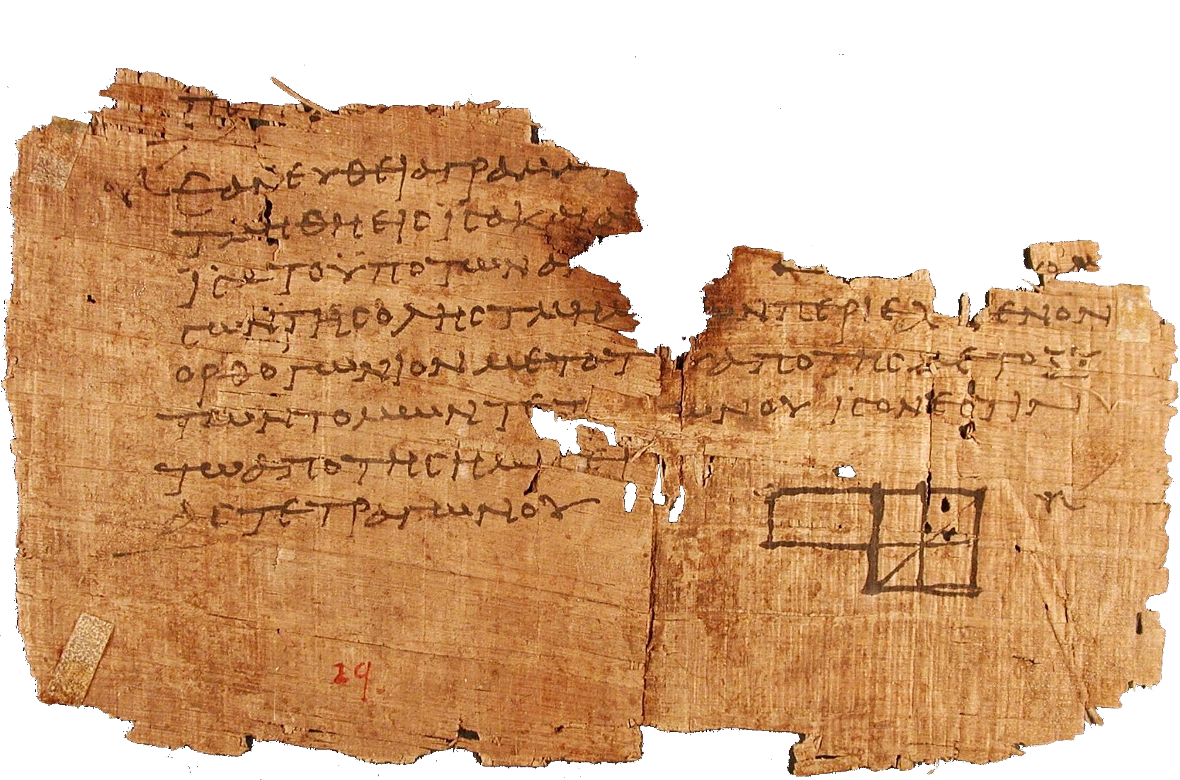
\includegraphics[width=\textwidth]{img/elements.png}}
	\only<2-4>{
	\only<2>{\centerline{Given a line $\ell$ and a point $P$ not lying on $\ell$, there exists}\centerline{\alert{one line through $P$ parallel to $\ell$.}}}
	\only<3>{\centerline{Given a line $\ell$ and a point $P$ not lying on $\ell$, there exists}\centerline{\alert{no line through $P$ parallel to $\ell$.}}}
	\only<4>{\centerline{Given a line $\ell$ and a point $P$ not lying on $\ell$, there exist}\centerline{\alert{at least two lines through $P$ parallel to $\ell$.}}}
	\vspace{\baselineskip}
	\begin{columns}[T,onlytextwidth]
	 \begin{column}{.33\textwidth}
	  \only<3>{
		\begin{alertbox}
		\centering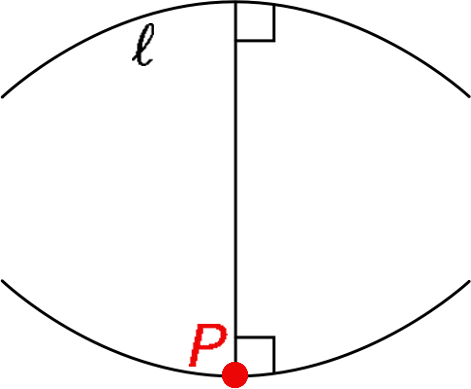
\includegraphics[width=\textwidth]{img/geo_elip.png}\\Elliptic
		\end{alertbox}
	  }
	  \only<4>{
		\begin{tbox}
		\centering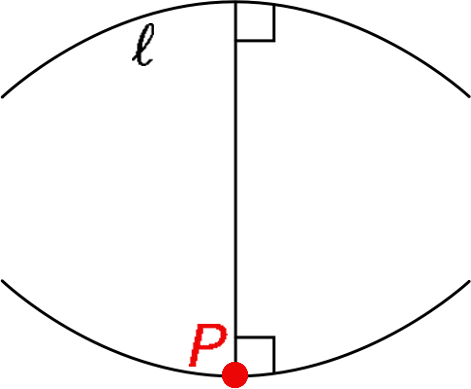
\includegraphics[width=\textwidth]{img/geo_elip.png}\\Elliptic
		\end{tbox}
	  }
	 \end{column}
	 \begin{column}{.34\textwidth}
	  \only<2>{
		\begin{alertbox}
			\centering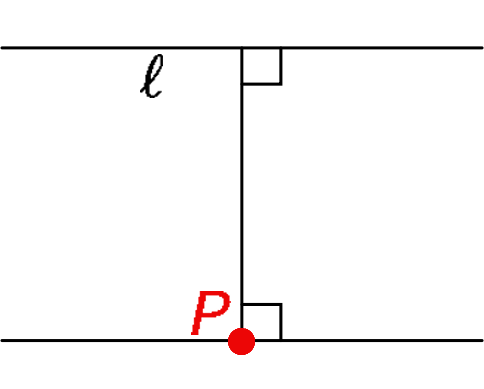
\includegraphics[width=\textwidth]{img/geo_eucl.png}\\Euclidean
		\end{alertbox}
	  }
	  \only<3-4>{
		\begin{tbox}
			\centering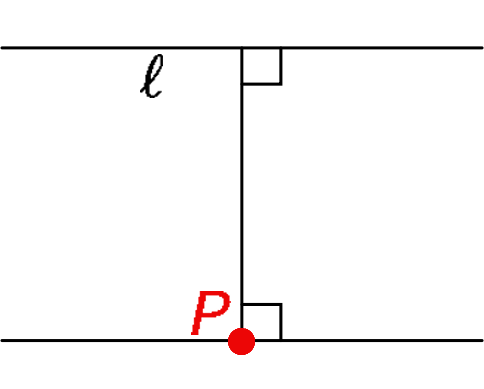
\includegraphics[width=\textwidth]{img/geo_eucl.png}\\Euclidean
		\end{tbox}
	  }
	 \end{column}
	 \begin{column}{.33\textwidth}
	  \only<4>{
		\begin{alertbox}
			\centering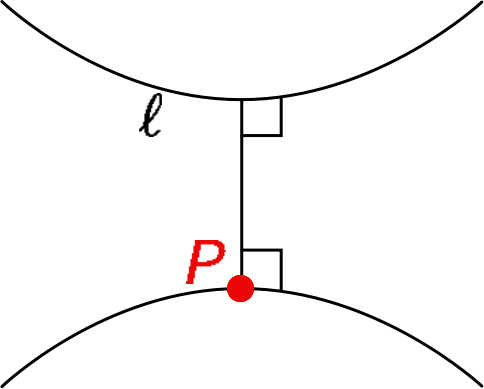
\includegraphics[width=\textwidth]{img/geo_hyp.png}\\Hyperbolic
		\end{alertbox}
	  }
	 \end{column}
	\end{columns}
	}
	\only<5->{
	\only<5>{\centerline{Given a line $\ell$ and a point $P$ not lying on $\ell$, there exist}\centerline{\alert{\textbf{?} many lines through $P$ parallel to $\ell$.}}}
	\only<6>{\centerline{\alert{Which axioms represent the truth?}}}
	\vspace{\baselineskip}
	\begin{alertbox}
	\begin{columns}[T,onlytextwidth]
	 \begin{column}{.33\textwidth}
		\centering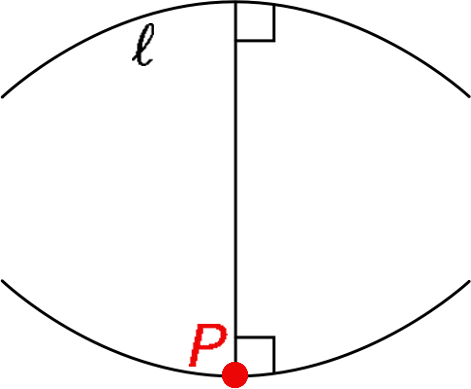
\includegraphics[width=0.73\textwidth]{img/geo_elip.png}\\Elliptic
	 \end{column}
	 \begin{column}{.34\textwidth}
		\centering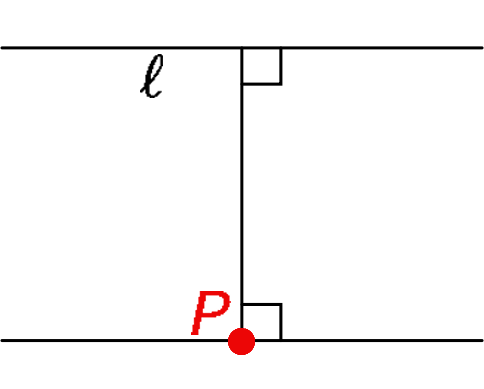
\includegraphics[width=0.73\textwidth]{img/geo_eucl.png}\\Euclidean
	 \end{column}
	 \begin{column}{.33\textwidth}
		\centering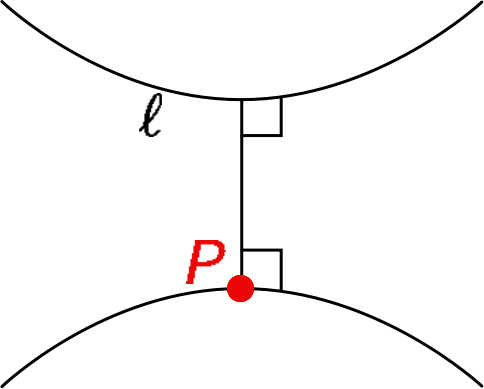
\includegraphics[width=0.73\textwidth]{img/geo_hyp.png}\\Hyperbolic
	 \end{column}
	\end{columns}
	\end{alertbox}
	}
\end{frame}
\begin{frame}{A Search for Foundations}
Axiomatisation of systems in the late 19th century
	\pause
	\begin{itemize}[<+->]
		\item Arithmetic of natural numbers by Peano
		\item Euclidean Geometry by Hilbert and Pasch
		\item Predicate logic by Frege
	\end{itemize}
	\pause[\thebeamerpauses]
	\centering \alert{Desire for a universal and consistent system}
\end{frame}
\begin{frame}{Cantor's Set Theory}
	\begin{columns}[c,onlytextwidth]
	 \begin{column}{.70\textwidth}
		\textit{``A set is a gathering together into a whole of definite, distinct objects of our perception or of our thought -- which are called elements of the set.''\nocite{cantor_set}\\\hfill-- Georg Cantor}
	 \end{column}
	 \begin{column}{.25\textwidth}
		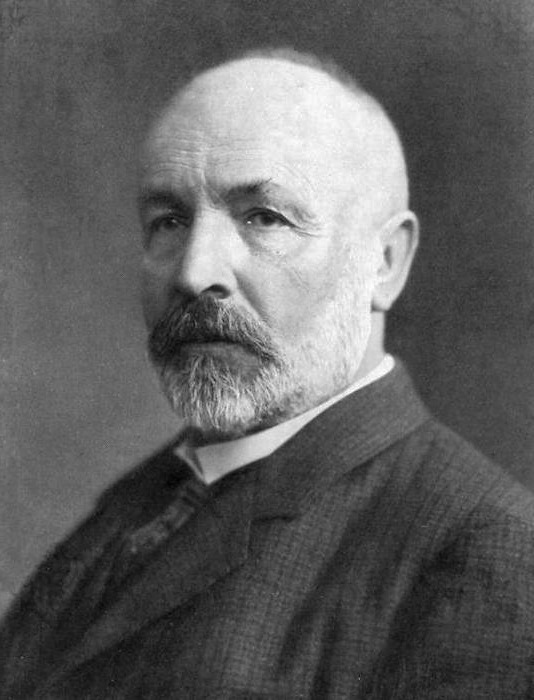
\includegraphics[width=\textwidth]{img/cantor.jpg}
	 \end{column}
	\end{columns}
	\vspace{\baselineskip}
	\pause
	\centerline{\alert{Certainly universal, but fairly naive.}}
\end{frame}
\begin{frame}{Frege's Logic System}
	\begin{columns}[c,onlytextwidth]
	 \begin{column}{.70\textwidth}
		Frege tried to build a consistent foundation by reducing mathematics to logic.
		\visible<2->{
		\begin{itemize}
			\item Sophisticated work, but not well received
		\end{itemize}}
	 \end{column}
	 \begin{column}{.25\textwidth}
		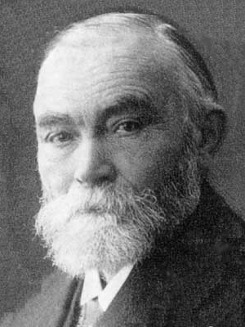
\includegraphics[width=\textwidth]{img/frege.jpg}
	 \end{column}
	\end{columns}
	\vspace{\baselineskip}
	\visible<3->{\centering Then one day, just before finishing his work, he received a letter from Russell\ldots}
\end{frame}
\begin{frame}{Russell's Paradox}
	Consider \emph{the set of all sets that are not members of themselves}:
	\begin{equation*}
		R\coloneqq\{X\mid X\notin X\}
	\end{equation*}\pause
	Question: Is R a member of itself? That is, does $R\in R$ hold?\pause\\
	\vspace{\baselineskip}
	Answer:\hspace{4.3em}$R\in R \iff R\notin R$, a contradiction!
\end{frame}
\begin{frame}{The Begin of the Crisis}
	\begin{columns}[c,onlytextwidth]
	 \begin{column}{.65\textwidth}
		Self-referentiality broke Cantor's and Frege's system.
	 \end{column}
	 \begin{column}{.3\textwidth}
		\centering
		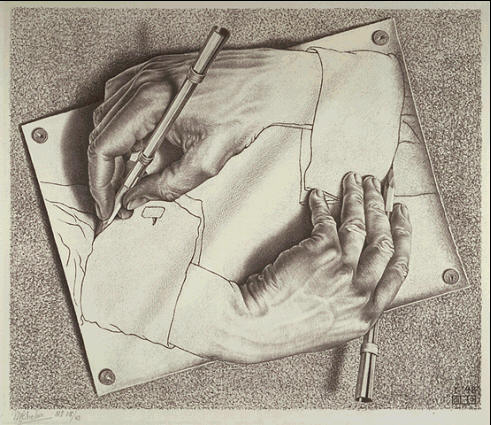
\includegraphics[width=\textwidth]{img/drawinghands.jpg}
	 \end{column}
	\end{columns}
	\pause
	\begin{quote}
		``Hardly anything more unfortunate can befall a scientific writer than to have one of the foundations of his edifice shaken after the work is finished.''\nocite{frege_appendix}\hfill-- Gottlob Frege
	\end{quote}
	\pause
	\centerline{\alert{A new foundation of mathematics had to be found.}}
\end{frame}
%------------------------------------------------
\section{The Foundational Crisis}
\begin{frame}{The Three Schools of Thought}
Three schools of thought tried to establish a new foundation.
\begin{itemize}
	\item Logicism
	\item Intuitionism
	\item Formalism
\end{itemize}
\vspace{.5\baselineskip}
\centering{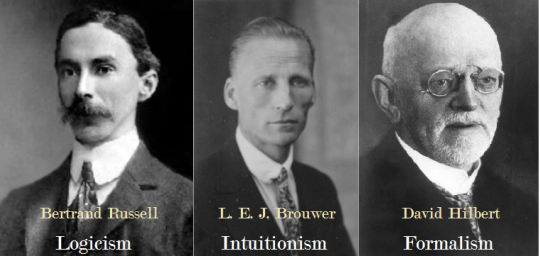
\includegraphics[height=0.42\textheight]{img/logic_intuit_form.png}}
\end{frame}
%------------------------------------------------
\subsection{Logicism}
\begin{frame}{A Foundation Made of Logic}
    \begin{itemize}
	\item<1-> Russell and Whitehead revisited Frege's idea of reducing mathematics to logic.	
	\item<3-> Only fundamentally logical laws are used as axioms.
	\begin{itemize}
		\item<4-> Justifications that used axioms are self-evident truths
	\end{itemize}
    \end{itemize}
    \visible<2->{\centering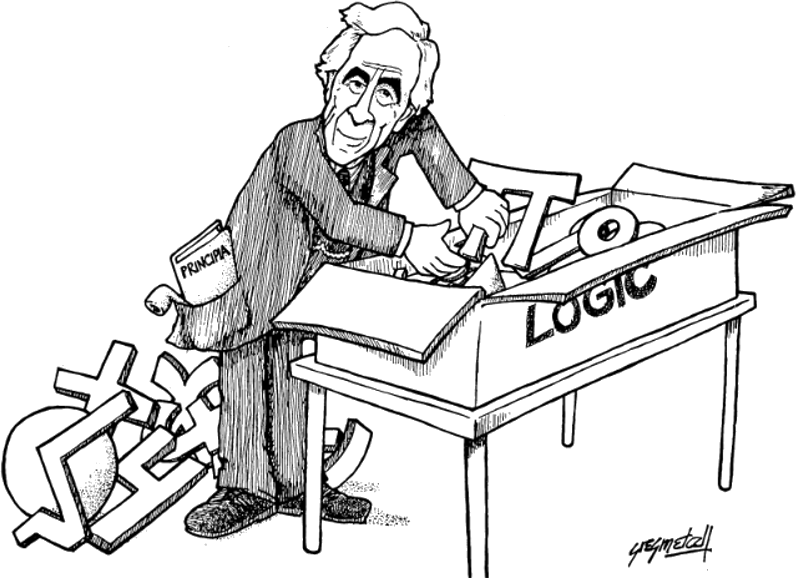
\includegraphics[height=0.5\textheight]{img/russell.png}}
\end{frame}
\begin{frame}{Principia Mathematica}
    \only<1-3>{
    \begin{itemize}[<+->]
	\item Type theory to avoid antinomies
	\item Difficulties in explaining some axioms
	\begin{itemize}
		\item<.-> Axiom of reducibility
		\item<.-> Axiom of infinity
	\end{itemize}
	\item Regarded as ``the outstanding example of an unreadable masterpiece''\nocite{math_experience} 
    \end{itemize}}
    \only<4>{
	\centerline{Principia Mathematica's infamous proof of $1+1=2$}
	\vspace{.5\baselineskip}
	\centering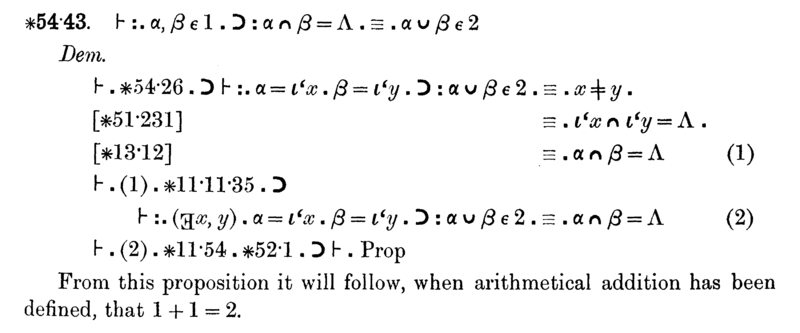
\includegraphics[width=\textwidth]{img/principia_mathematica.png}}
\end{frame}
%------------------------------------------------
\subsection{Intuitionism}
\begin{frame}{Proofs with Real Evidence}
	\vspace{\baselineskip}
	\begin{columns}[T,onlytextwidth]
	 \begin{column}{.65\textwidth}
	    \begin{itemize}
		\item<1-> Mathematics is a constructive process conducted by humans.
		\item<3-> The existence of an object is equivalent to the possibility of its construction.
		\item<4-> Consequently, some assumptions of classical logic must be rejected.
	    \end{itemize}
	 \end{column}
	 \begin{column}{.3\textwidth}
		\centering
		\visible<2->{\centering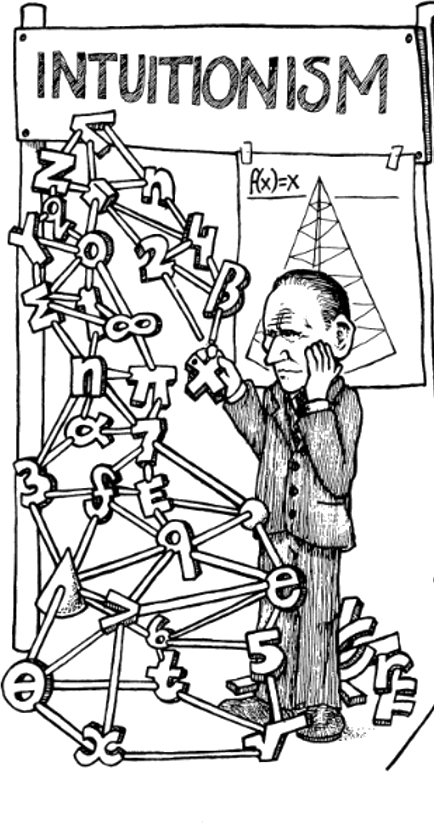
\includegraphics[width=\textwidth]{img/brouwer.png}}
	 \end{column}
	\end{columns}
\end{frame}
\begin{frame}{$P\lor\lnot P\equiv\ $\textbf{?}}
Intuitionists reject the \emph{law of excluded middle}:
\begin{quote}
	For any proposition P, either P or its negation is true.
\end{quote}
	\pause
	\textbf{Proposition:} There exist two irrational numbers $a$ and $b$ such that $a^b$ is rational.\\\pause
	\vspace{\baselineskip}
	\textbf{Proof.} It is known that $\sqrt{2}$ is irrational. Let us consider the number $\sqrt{2}^{\sqrt{2}}$.\pause$ $ If it is rational, our statement is proved.\pause$ $ If it is irrational, $(\sqrt{2}^{\sqrt{2}})^{\sqrt{2}}=2$ proves our statement.\hfill$\qed$
\end{frame}
\begin{frame}{What a Hassle!}
Intuitionistic logic complicates many proofs.
\pause
\begin{quote}
``Taking this tertium non datur (law of excluded middle) from the mathematician would be the same as, say, denying the astronomer his telescope and the boxer the use of his fists.''\nocite{hilbert_tertium_non_datur}\\\hfill-- David Hilbert
\end{quote}
\begin{columns}[c,onlytextwidth]
\begin{column}{.15\textwidth}
\vspace{0.1\baselineskip}
\visible<2->{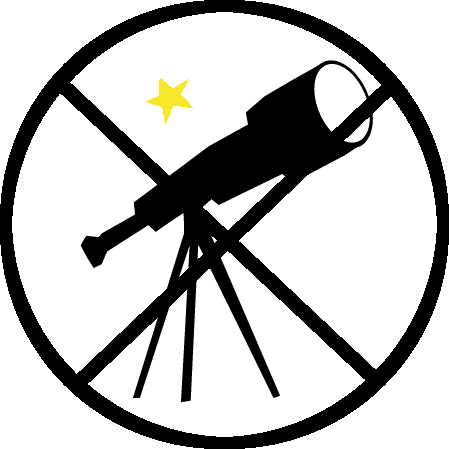
\includegraphics[width=\textwidth]{img/telescope.png}}
\end{column}
\begin{column}{.65\textwidth}
\vspace{0.1\baselineskip}
\visible<3->{\centering \alert{Only a few scholars adhered to intuitionism.}}
\end{column}
\begin{column}{.15\textwidth}
\vspace{0.1\baselineskip}
\visible<2->{
\includegraphics[width=\textwidth]{img/boxinggloves.png}}
\end{column}
\end{columns}
\end{frame}
%------------------------------------------------
\subsection{Formalism}
\begin{frame}{Mathematics as a Symbolic Game}
	\vspace{\baselineskip}
	\begin{columns}[T,onlytextwidth]
	 \begin{column}{.65\textwidth}
	    \begin{itemize}
		\item<1-> Mathematics shall be based on symbols and axioms that describe syntactic operations on symbols.
		\item<3-> Mathematics does not need to justify the existence of its objects since its objects are just meaningless shapes.
		\item<4-> The system's consistency must be verified.
	    \end{itemize}
	 \end{column}
	 \begin{column}{.3\textwidth}
		\centering
		\visible<2->{\centering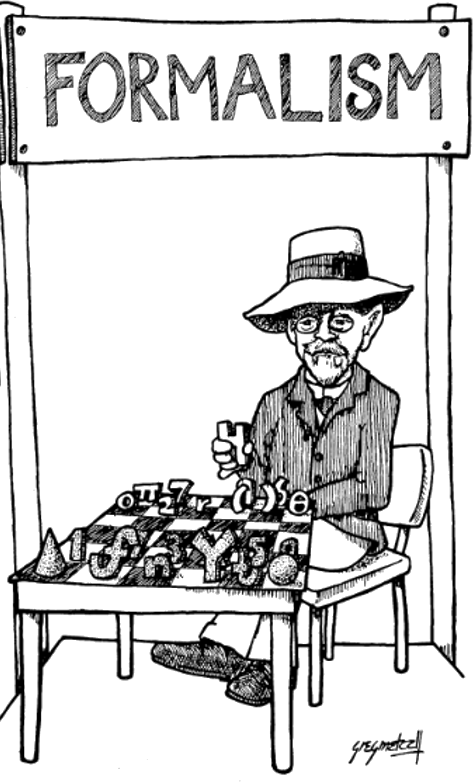
\includegraphics[width=\textwidth]{img/hilbert.png}}
	 \end{column}
	\end{columns}
\end{frame}
\begin{frame}{Hilbert's Programme}
\emph{Hilbert's programme} consists of two steps:
\pause
\begin{enumerate}[<+->]
	\item Formalise a system that is able to derive all of mathematics using syntactical operations
	\item Prove the system's consistency with metamathematical reasoning
\end{enumerate}
\visible<4>{\centerline{\alert{The dream of a complete and consistent mathematical system}}}
\end{frame}
%------------------------------------------------
\subsection{Peak and End}
\begin{frame}{The Peak of the Crisis}
In 1928, the peak of the crisis was reached.
\pause
    \begin{itemize}[<+->]
	\item Brouwer boycotted the \textit{International Congress of Mathematicians}.
	\item Hilbert excluded Brouwer as a co-publisher from the journal ``Mathematischen Annalen''.
	\item Brouwer stopped publishing intuitionistic articles.
    \end{itemize}
\pause[\thebeamerpauses]
Optimism for a complete and consistent formal system grew\ldots
\end{frame}
\begin{frame}{The End of the Crisis}
\vspace{\baselineskip}
\begin{columns}[c,onlytextwidth]
 \begin{column}{.75\textwidth}
\ldots but then came Gödel.\\
\visible<2->{In 1931, he ended the crisis with his two \emph{incompleteness theorems}.}
 \end{column}
 \begin{column}{.25\textwidth}
  \centering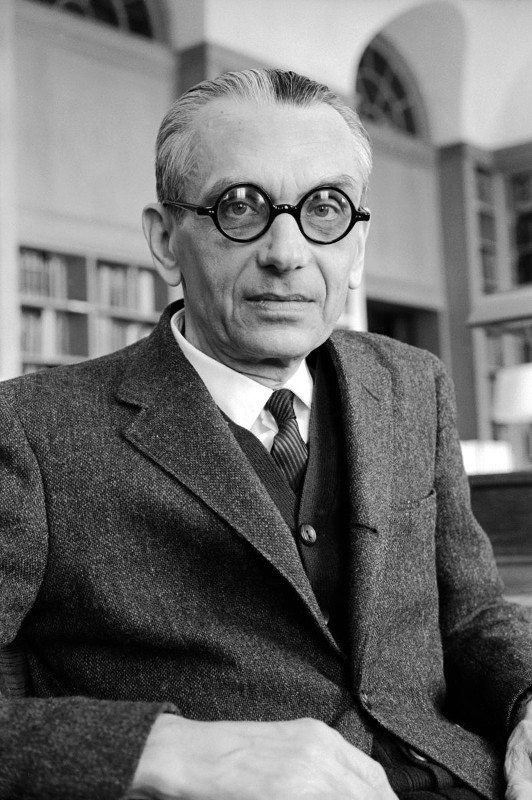
\includegraphics[height=0.35\textheight]{img/goedel.jpg}
 \end{column}
\end{columns}
	\visible<3->{\small{\begin{theorem}[First Incompleteness Theorem] Any consistent formal system within which a certain amount of elementary arithmetic can be carried out is incomplete.\end{theorem}}}
	\visible<4->{\small{\begin{theorem}[Second Incompleteness Theorem] Any consistent formal system within which a certain amount of elementary arithmetic can be carried out cannot prove its own consistency.\end{theorem}}}
\end{frame}
%------------------------------------------------
\section{Aftermath and Prospects}
\begin{frame}{Modern Mathematics}
To this day, formalism poses the foundation of mathematics.
\pause
\begin{itemize}
	\item Zermelo-Fraenkel set theory (ZFC) as established foundation
\end{itemize}
\pause
Most mathematicians do not deal with foundational research.
\pause
\begin{quote}
``The typical working mathematician is a Platonist on weekdays and a formalist on Sundays.''\nocite{math_experience}\\\hfill-- The Mathematical Experience
\end{quote}
\end{frame}
\begin{frame}{The Next Crisis?}
Digitisation of mathematics
\pause
    \begin{itemize}[<+->]
	\item Some see it as an inevitable enrichment; others face it with distrust.
	\item Can we trust proofs by computers?
    \end{itemize}
\pause[\thebeamerpauses]
\vspace{\baselineskip}
\centerline{\Large\alert{Are we part of the next mathematical crisis?}}
\end{frame}
%------------------------------------------------
\begin{frame}
	\center
	\Large{Thanks for your attention! Any questions?}
	\vspace{0.5\baselineskip}\\
	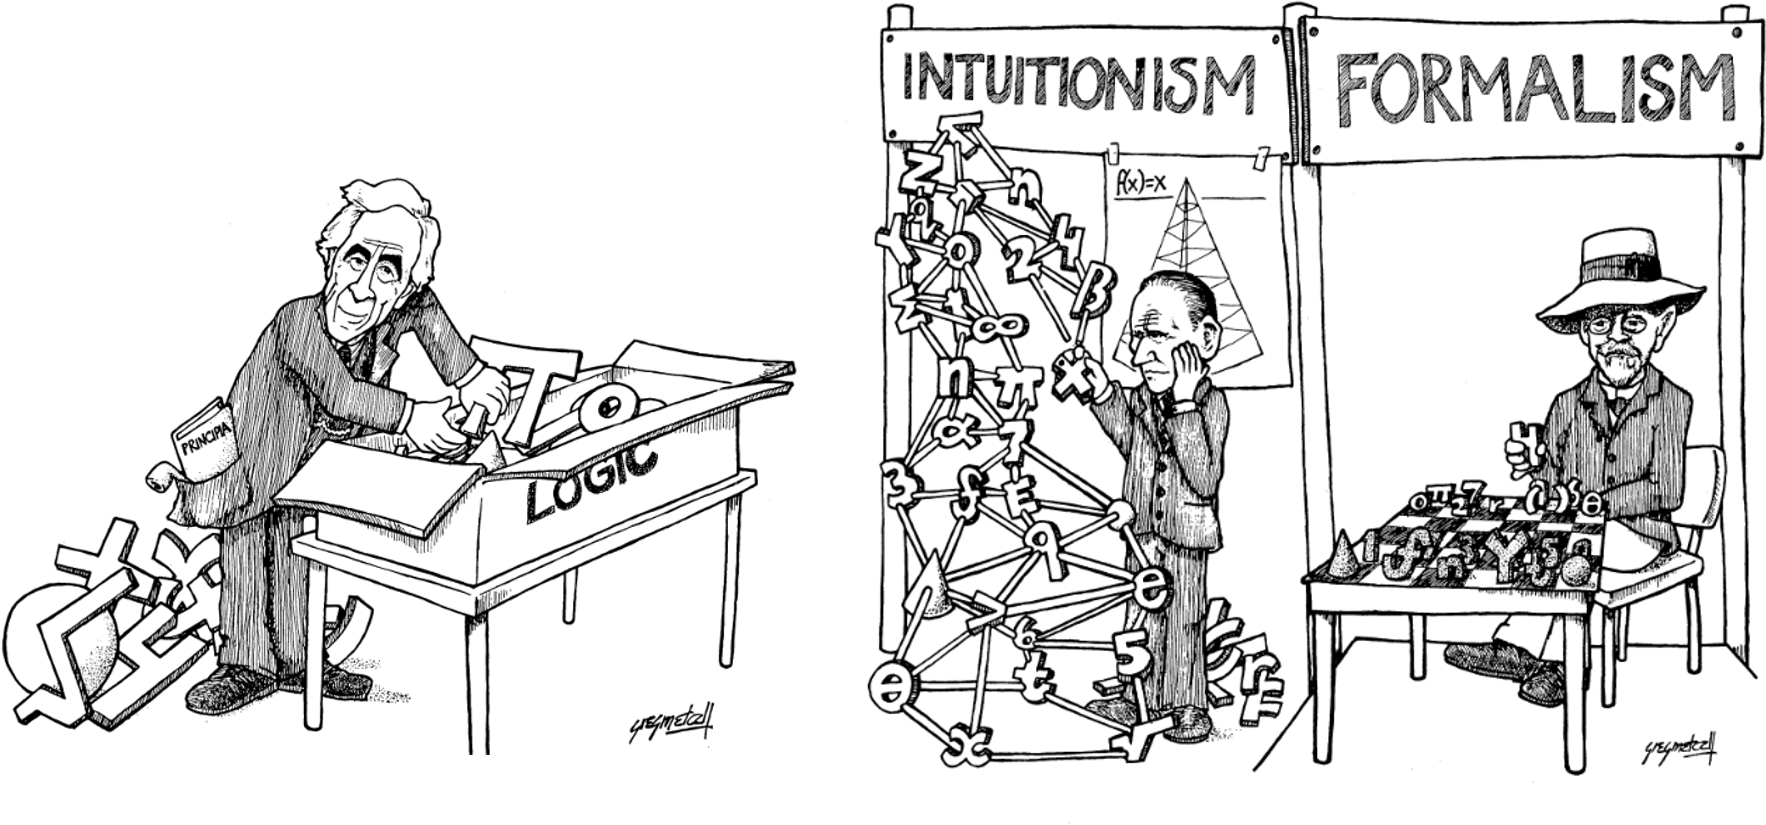
\includegraphics[height=0.6\textheight]{img/logic_intuit_form2.png}
\end{frame}
%----------------------------------------------------------------------------------------
\begin{frame}[allowframebreaks]{References}
  \bibliography{../paper/sources.bib}
  \bibliographystyle{abbrv}
\end{frame}

\begin{frame}[allowframebreaks]{Image Sources}
\begin{itemize}
\item Euclid's Elements: \url{math.ubc.ca/~cass/Euclid/papyrus/tha.jpg}
\item Geometries: \url{upload.wikimedia.org/wikipedia/commons/thumb/7/78/Noneuclid.svg/2000px-Noneuclid.svg.png}
\item Cantor: \url{upload.wikimedia.org/wikipedia/commons/e/e7/Georg_Cantor2.jpg}
\item Frege: \url{nndb.com/people/523/000179983/gottlob-frege-2-sized.jpg}
\item Drawing Hands: \url{mcescher.com/wp-content/uploads/2013/10/LW355-MC-Escher-Drawing-Hands-1948.jpg}
\item Schools of Thought: \url{geopolicraticus.tumblr.com/post/142561195372}
\item Schools of Thought (comic): \url{maa.org/sites/default/files/pdf/upload\_library/22/Allendoerfer/1980/0025570x.di021111.02p0048m.pdf}
\item Gödel: \url{newyorker.com/tech/elements/waiting-for-godel}
\end{itemize}
\end{frame}

\end{document} 
